\section{Experiments on synthetic data}

We present results on two sets of synthetic data experiments.

\subsection{Deblending two stars}

We set up an experiment to study the
ability of StarNet to deblend two simulated stars.
On a $20\times20$ pixel image,
we simulate two stars of equal flux at distance $\delta$ pixels apart, and
examine the approximate posterior produced by StarNet (Figure~\ref{fig:deblending_fig}).
We generate the stars with the DECam PSF, which 
has a full width at half maximum 
(defined as twice the radius at which the PSF is half its peak brightness) of 4.2 pixels. 
The threshold of near-perfect deblending is a distance of $\delta = 1.5$ pixels, which is less than half the PSF 
full width at half maximum. 

\begin{figure}[tb]
    \centering
    \begin{subfigure}{0.8\textwidth}
        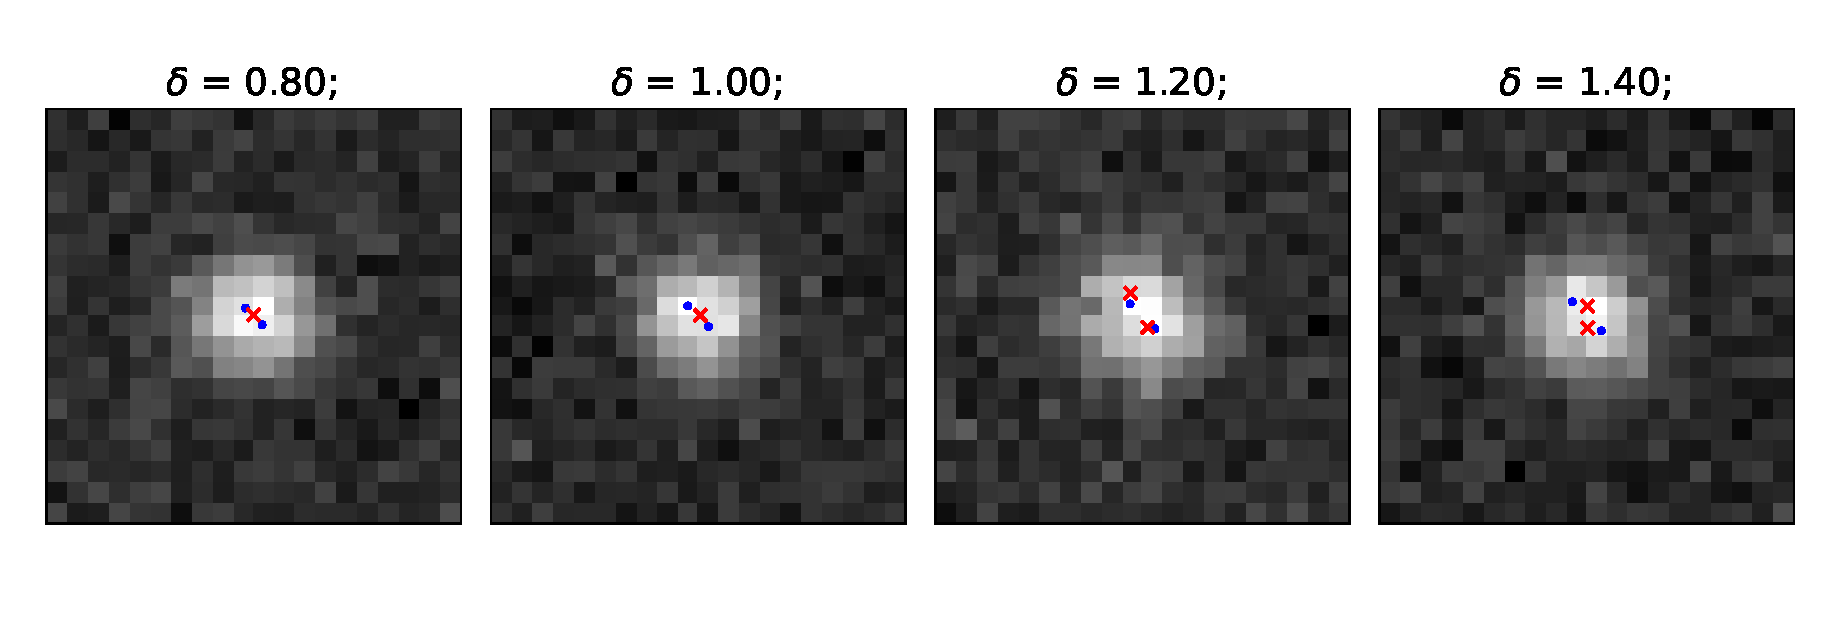
\includegraphics[width=\textwidth]{figures_vg/deblending/example_deblending.eps}
    \end{subfigure}
    \begin{subfigure}{0.8\textwidth}
        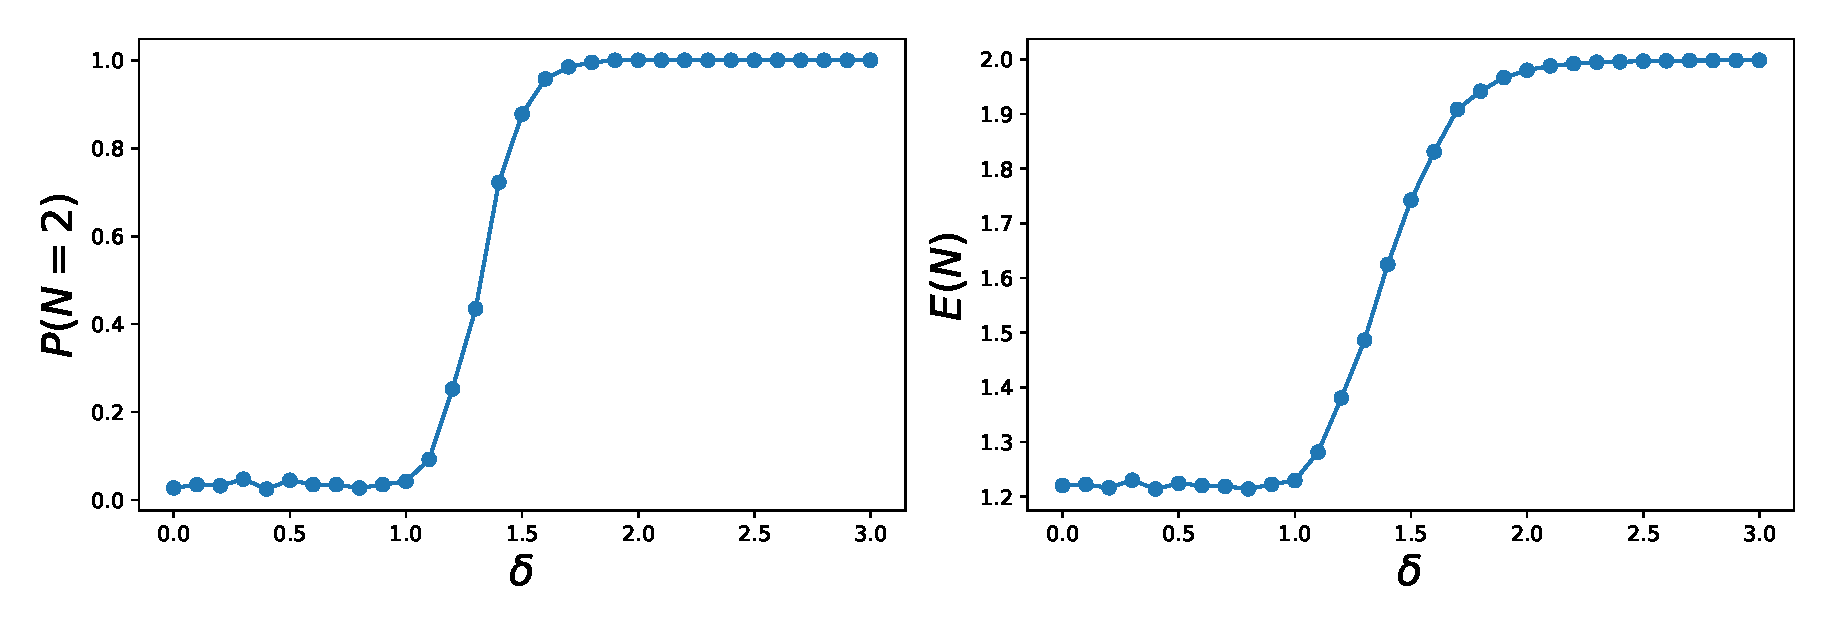
\includegraphics[width=\textwidth]{figures_vg/deblending/summary_statistics.eps}
    \end{subfigure}
    \caption{(Top row) Simulated images with two stars separated by distance $\delta$ in pixels.
    True locations are in blue. StarNet MAP locations in red. 
    In these examples,tiles the StarNet MAP catalog correctly contains two stars when separated by $\delta \geq 1.2$,
    but only estimated one star when $\delta \leq 1$.
    (Bottom left) The probability that $N$, the number of sources in the image, equals two
    under the variational posterior, as $\delta$ varies.
    (Bottom right) The expectation of $N$ under the variational posterior as $\delta$ varies. }
    \label{fig:deblending_fig}
\end{figure}

\subsection{Coverage of credible intervals}
\label{sec:coverage}

We have seen that on M2, the StarNet 95\% posterior interval did not contain the ground truth number of stars (Section~\ref{sec:results_on_m2}).
On M2, we attribute this to model mis-specification, specifically due to an imperfectly
estimated background.

We check the coverage of StarNet posterior intervals on synthetic data
to reveal any issues other than model mis-specification that may explain these results.
We sample a single $100\times100$ pixel image from the generative model. 
On this sampled image, the true number of stars, $N = 1195$,
is still considerably smaller than the 0.01-th percentile of
the approximate posterior distribution (Figure~\ref{fig:starnet_density}).


\begin{figure}[tb]
    \centering
    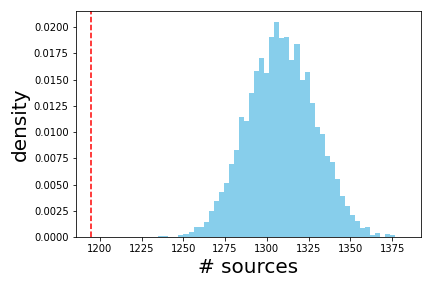
\includegraphics[width=0.45\textwidth]{./figures/coverage/starnet_histogram.png}
    %\vspace{-0.4cm}
    \caption{Distribution of 5000 samples of the number of sources from the StarNet approximate posterior.
    The true number of sources demarcated in red. }
    \label{fig:starnet_density}
\end{figure}

We attribute this over-estimation to the spatial independence of the approximate posterior.
Specifically, StarNet \textit{overestimates} the number of sources close to tile boundaries.
Heuristically, for a
a source located in the interior of the tile
within $\epsilon$ of a boundary (but still far from a corner),
StarNet should assign a probability of $\frac{1}{2}$ for
having one source, and a probability $\frac{1}{2}$ for having none, as $\epsilon \rightarrow 0$.
Should this be the case, then over the entire image, which consist of many tiles,
a source on a tile boundary is correctly accounted for: it has a 50-50 chance of being assigned to one tile or another
in the approximate posterior, and this source contributes 
a count of one to the posterior expectation on the number of stars. 

However, we observe empirically that as a source approaches the edge of a tile,
the posterior probability that $N = 1$ approaches a number
slightly \textit{larger} than $\frac{1}{2}$ (Figure~\ref{fig:starnet_edges}).
Therefore, the approximate posterior overestimates the expected number of sources in the full image.

To illustrate the effect of tiles, we simulate images with the constraint that all sources are at least 0.1-pixels from all tile edges. 
In this case, then the StarNet approximate posterior has much closer to correct coverage (Figure~\ref{fig:coverage_good})

\begin{figure}[tb]
    \centering
    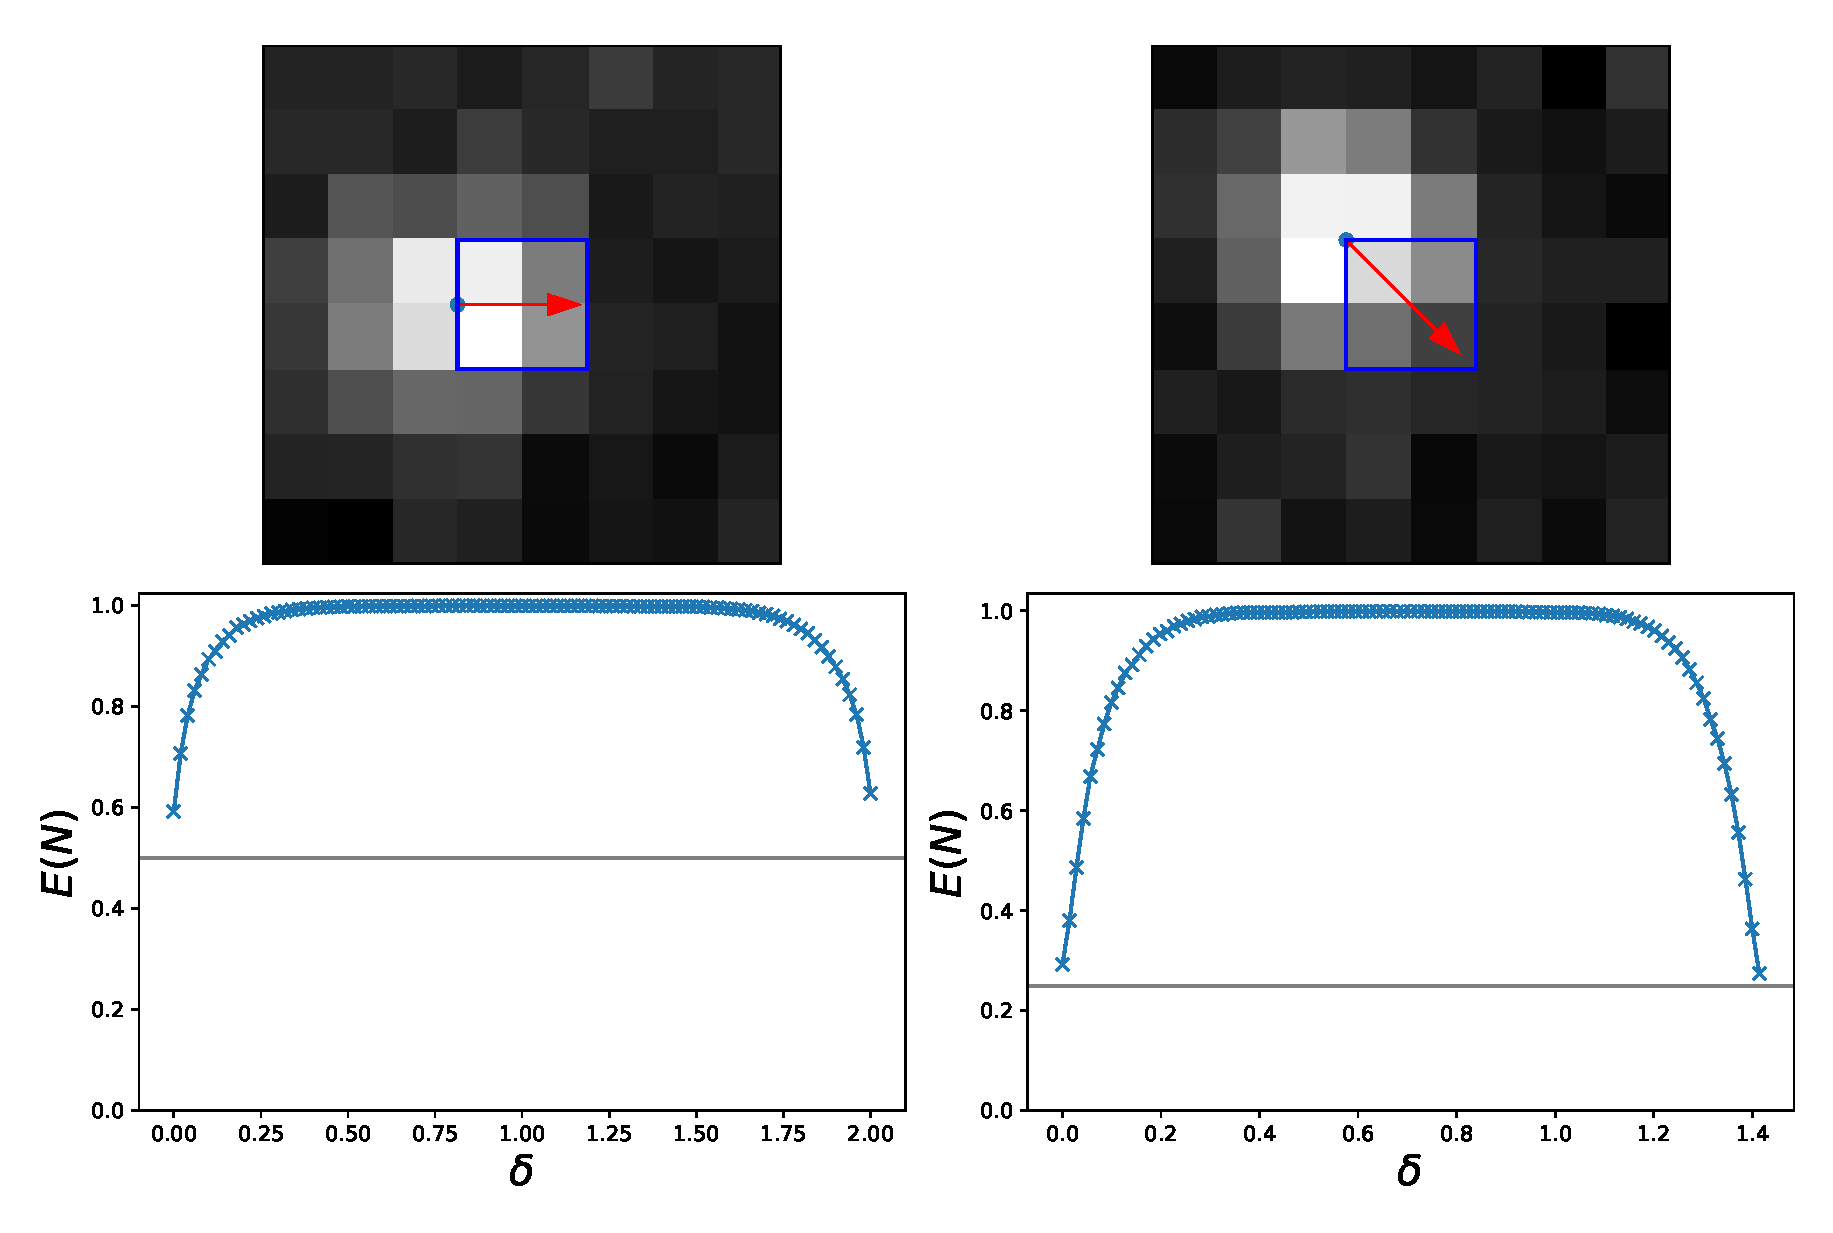
\includegraphics[width=0.8\textwidth]{./figures_vg/coverage/edges_example.eps}
    %\vspace{-0.4cm}
    \caption{The expected number of sources under the StarNet approximate posterior as a function of distance from the edge (in pixels).
    On the left, we place a star on the left-most edge, and move its location $\delta$ pixels to the right.
    On the right, we place a star on the top-left corner, and move its location $\delta$ pixels towards the bottom-right corner.}
    \label{fig:starnet_edges}
\end{figure}

\begin{figure}[tb]
    \centering
    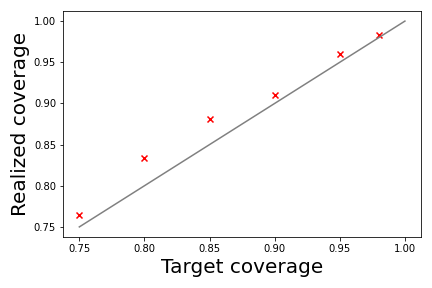
\includegraphics[width=0.5\textwidth]{./figures/coverage/good_coverage.png}
    %\vspace{-0.4cm}
    \caption{Coverage test in simulated $100\times100$ images where all true stars are constrained to be 0.1-pixels away from any tile
    boundary.
    We simulate 1000 images from the prior and generative model, and for each image, we compute a $(1 - \alpha)$-level posterior interval for the number of stars by taking the $\frac{\alpha}{2}$ and $(1 -\frac{\alpha}{2})$-th percentiles of 5000 StarNet posterior samples.
    For each $\alpha$, we plot the observed coverage against the target $(1 - \alpha)$-level coverage. }
    \label{fig:coverage_good}
\end{figure}

\subsection{Effects of padding}
We study the effect of padding the input 
tiles to the StarNet neural network architecture. 
We re-visit the investigation of tile boundary effects 
described in the subsection above, where 
we simulate a source closer and closer to the tile boundary. 
The experiments above used the M2 network, 
which uses $2\times 2$ tiles and three pixels of padding. 
With only one pixel of padding, sources become even more 
over-estimated on tile edges (Figure~\ref{fig:starnet_edges_lesspad}). 

\begin{figure}[tb]
    \centering
    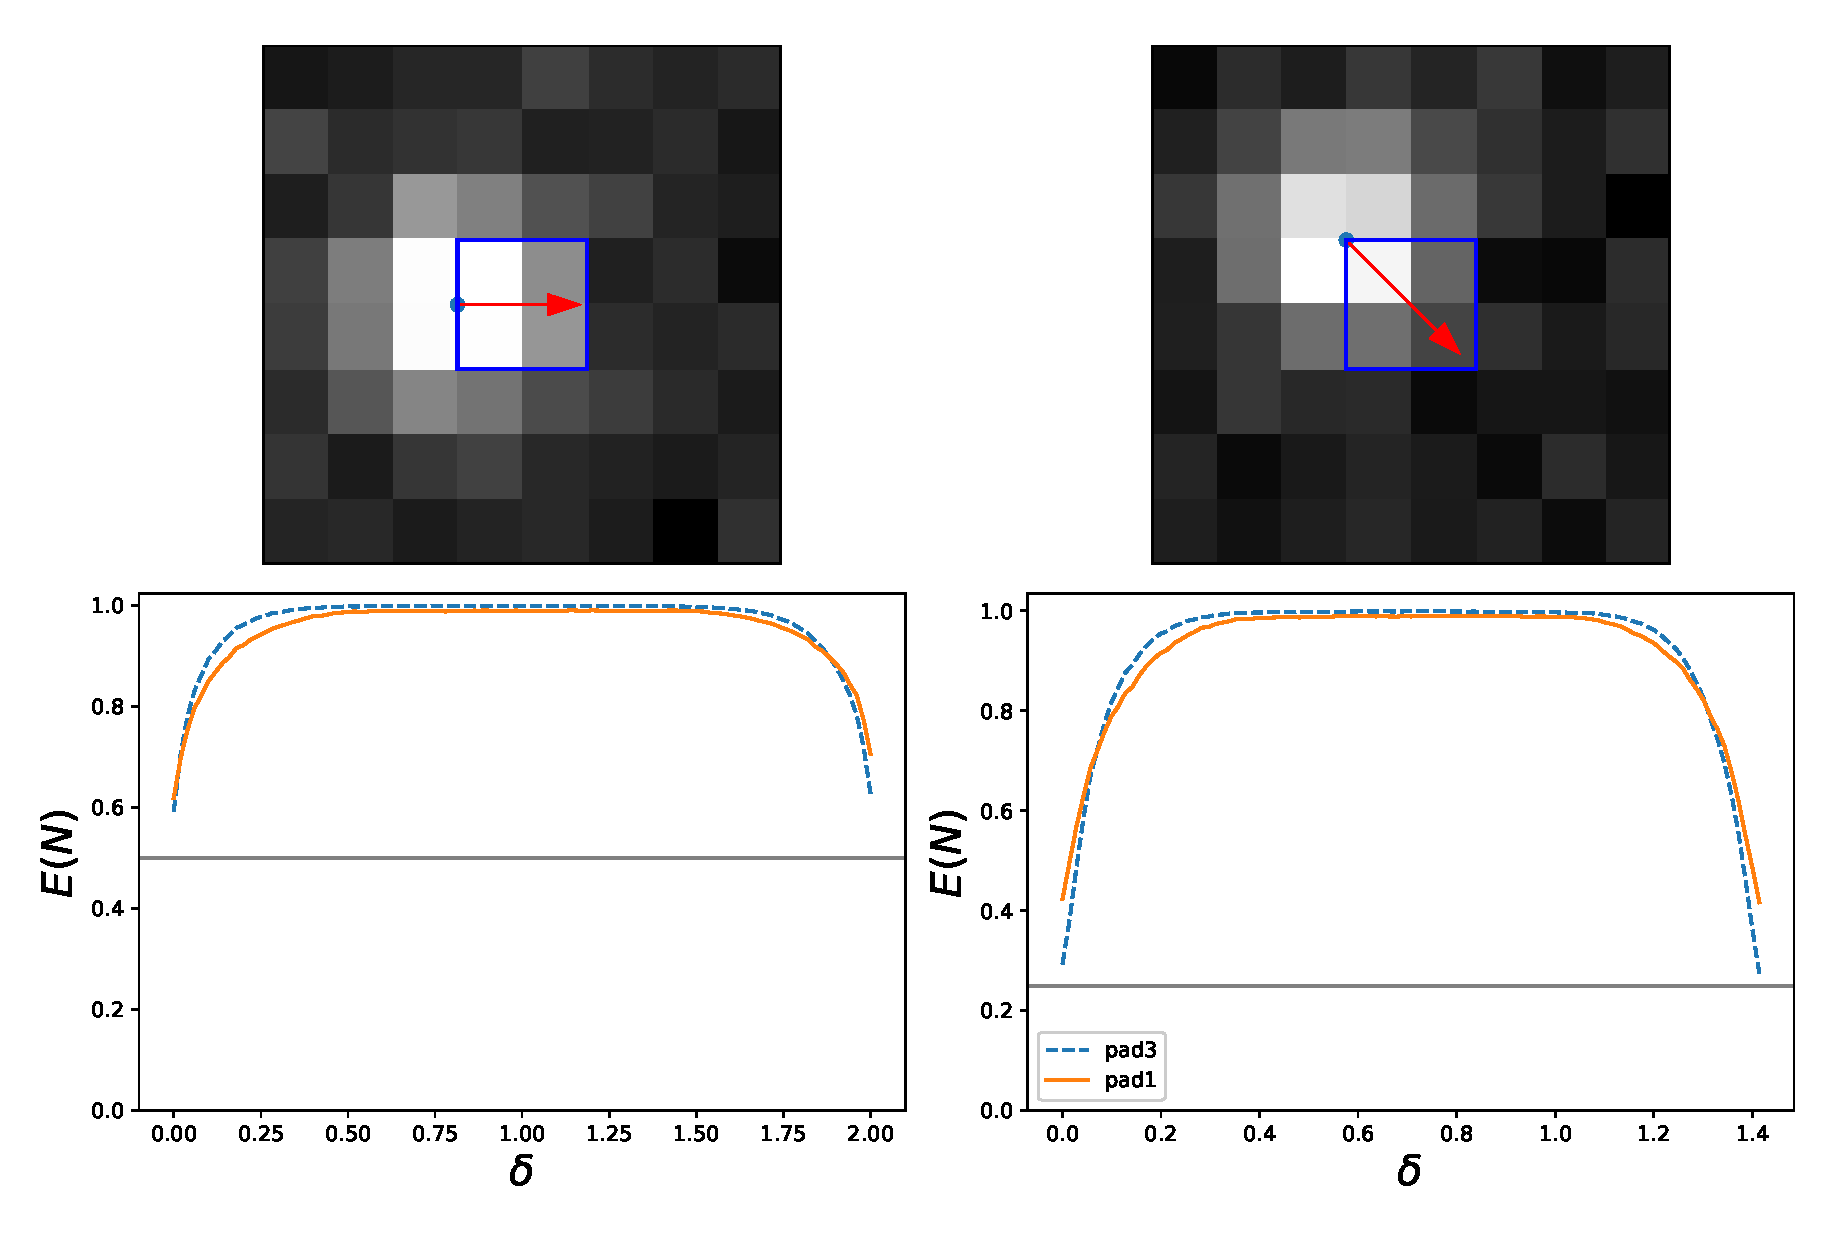
\includegraphics[width=0.8\textwidth]{./figures_vg/coverage/edges_example_lesspad.eps}
    %\vspace{-0.4cm}
    \caption{The same experimental setup as Figure~\ref{fig:starnet_edges}, but we 
    study the effect of padding the neural network input tiles. 
    In dashed blue, the posterior when 
    StarNet uses three pixels of padding. 
    In solid orange, the posterior when only one pixel of padding is used.
    }
    \label{fig:starnet_edges_lesspad}
\end{figure}
